\documentclass[border=6pt]{standalone}
\usepackage{tikz}
\usetikzlibrary{arrows.meta,calc}
\begin{document}
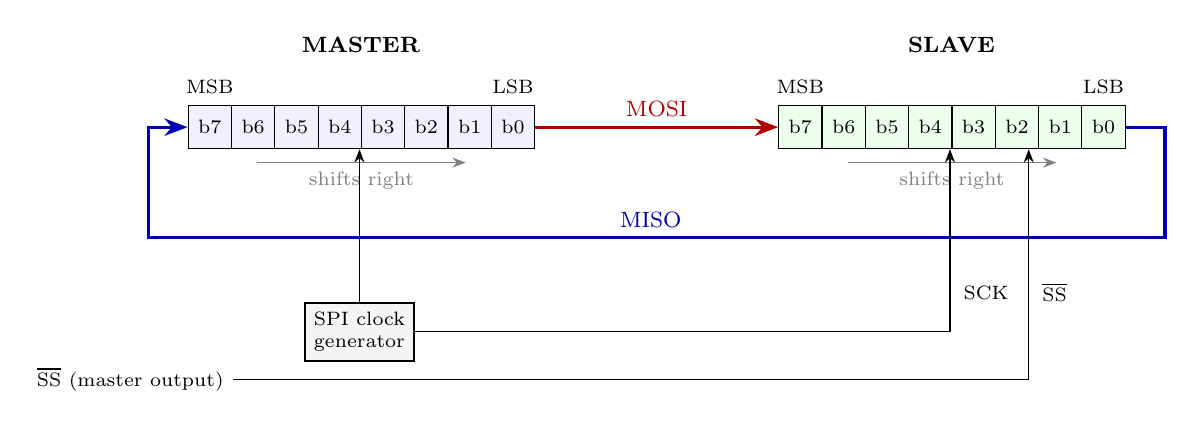
\begin{tikzpicture}[>=Stealth,font=\small,
 cell/.style={draw,minimum width=0.55cm,minimum height=0.55cm,inner sep=0,font=\scriptsize}]
% master register cells b7..b0 at x = 0..3.85
\foreach \i in {0,...,7} {
  \pgfmathtruncatemacro{\b}{7-\i}
  \node[cell,fill=blue!6] (m\i) at (\i*0.55,0) {b\b};
  \node[cell,fill=green!8] (s\i) at (7.5+\i*0.55,0) {b\b};
}
\node[font=\footnotesize\bfseries] at (1.92,1.05) {MASTER};
\node[font=\footnotesize\bfseries] at (9.42,1.05) {SLAVE};
\foreach \p/\x in {m/0,s/7.5} {
  \node[font=\scriptsize,anchor=south] at (\x,0.3) {MSB};
  \node[font=\scriptsize,anchor=south] at (\x+3.85,0.3) {LSB};
  \draw[->,gray] (\x+0.6,-0.45) -- (\x+3.25,-0.45) node[midway,below,font=\scriptsize]{shifts right};
}
% MOSI: master LSB out -> slave MSB in
\draw[->,very thick,red!70!black] (m7.east) -- (s0.west) node[pos=0.5,above,font=\footnotesize]{MOSI};
% MISO: slave LSB out -> master MSB in
\draw[->,very thick,blue!70!black] (s7.east) -- ++(0.5,0) -- ++(0,-1.4) -| ($(m0.west)+(-0.5,0)$) -- (m0.west);
\node[font=\footnotesize,blue!70!black,anchor=south] at (5.6,-1.4) {MISO};
% clock and SS
\node[draw,thick,fill=gray!8,align=center,font=\scriptsize] (clk) at (1.9,-2.6) {SPI clock\\generator};
\draw[->] (clk.east) -- (9.4,-2.6) -- (9.4,-0.28);
\node[font=\scriptsize,anchor=west] at (9.45,-2.1) {SCK};
\draw[->] (clk.north) -- (1.9,-0.28);
\draw[->] (0.3,-3.2) node[left,font=\scriptsize]{$\overline{\mathrm{SS}}$ (master output)} -- (10.4,-3.2) -- (10.4,-0.28);
\node[font=\scriptsize,anchor=west] at (10.45,-2.1) {$\overline{\mathrm{SS}}$};
\end{tikzpicture}
\end{document}
